\subsubsection{Stable Diffusion} \label{sec:stable-diffusion}

Stable Diffusion \cite{rombach_high-resolution_2021} rose from the idea of democratization high-resolution images. According to the original paper, high-end models demand hundreds of thousands of dollars to be trained solely due to their complexities. These models generally operate directly on the pixel space. The training and evaluation of such models necessitate significant computational resources, which are typically only available to the largest companies, thereby contributing to significant carbon footprints.

They apply the diffusion process (see Section \ref{sec:diffusion}) in pre-trained \acp{AE}' (Section \ref{sec:autoencoders}) latent space to optimize the diffusion model practice instead of directly on the pixel space.

For this stable diffusion model, training is separated into two phases: the training of the \ac{AE} and the training of the diffusion model.

One needs the text and Gaussian noise to infer new images given text. The text is embedded using a transformer (see Section \ref{sec:transformers}). In order to increase the relation between the text and the generated image, the text embeddings for an empty string are also generated.

The model takes the initial noise, text and audio embeddings, and timestamp as inputs. Through inverse diffusion process, it generates two new images: one conditioned on the real embeddings, and another with no embeddings (empty string embedding). The image generated by the real embeddings is a synthesis conditioned on the given text and audio input. On the other hand, generating an image without any embeddings produces a random image unconditioned by the provided text or audio. At each step of diffusion process, the model compares the two images to evaluate their differences. By increasing this difference, the final output image becomes conditioned on the initial textual input to a greater extent.

The U-Nets in the diffusion process use cross-attention mechanisms for their respective embeddings (refer to Section \ref{sec:u-net}). Cross-attention extends attention mechanisms used in neural networks. Self-attention captures relationships within a single sequence or embedding, while cross-attention captures dependencies between different sequences or embeddings.

In this study, the U-Nets use cross-attention to allow information exchange and interaction between audio features and other modalities, including text embeddings or image representations. Using cross-attention in the diffusion process improves the model's ability to consider local and global contextual cues from multiple sources during audio synthesis.

Using cross-attention allows different parts of the network to attend to each other's information, enabling better integration and coherence across various modalities involved in generating soundscapes from textual input. This comprehensive modeling improves the overall performance.

After the diffusion process is completed, the decoder takes the generated image embeddings and generates a new image.

This process can be seen in Figure \ref{fig:stable-diffusion}.

\begin{figure}[ht]
    \centering
    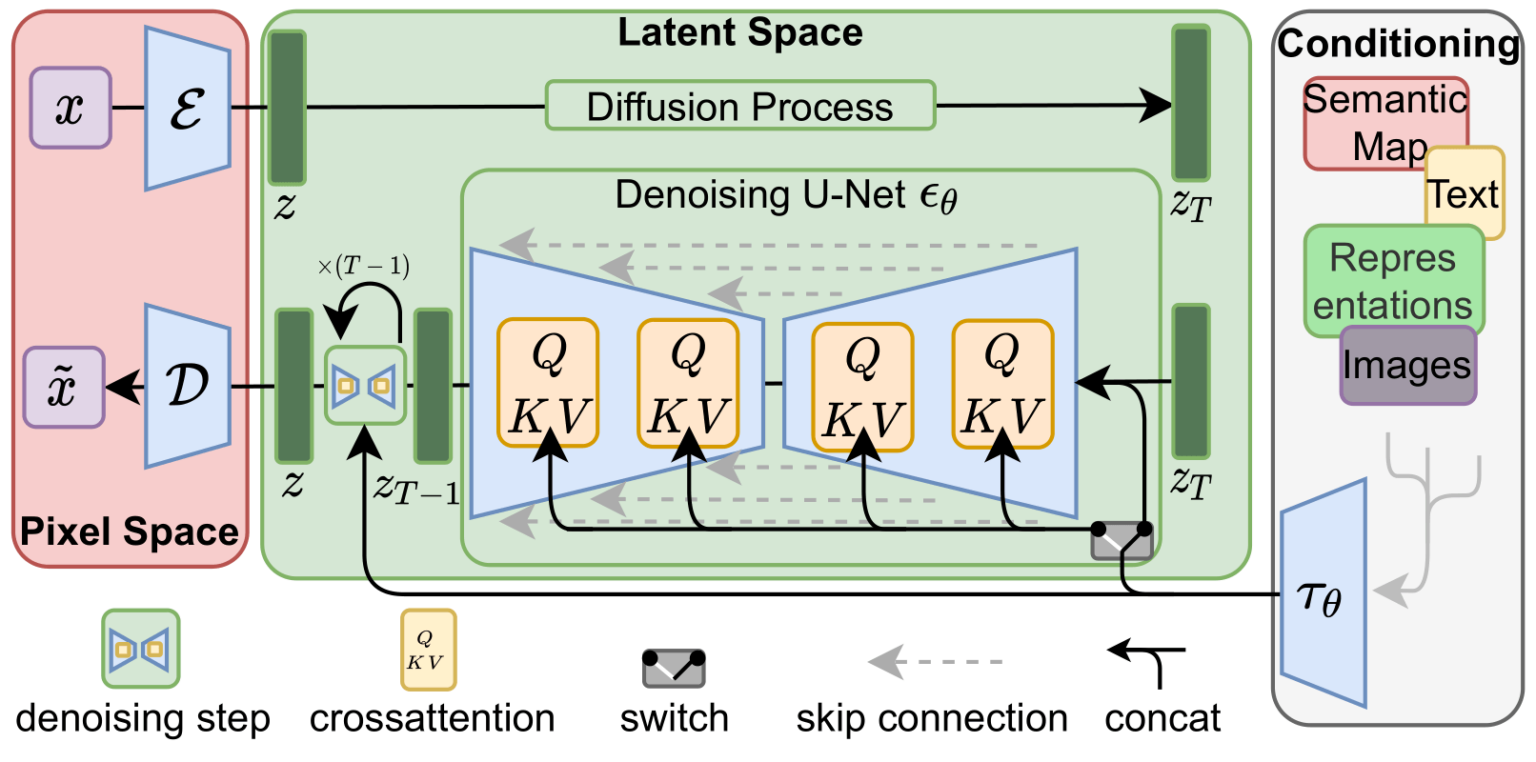
\includegraphics[width=\textwidth]{figures/2-sota/stable-diffusion.png}
    \caption[Stable diffusion architecture]{\textbf{Stable diffusion architecture} --- The Figure was taken from the original paper. On the top left, the original image $x$ is encoded with the \ac{AE}, and the diffusion process happens with the encodings. The text (or another data kind) is encoded with a transformer $\tau_{\theta}$, and these encodings are applied with attention to the denoising U-Nets. This denoising U-Net is applied $T$ times before the decoder transforms the encodings into an actual image in the pixel space again.}
    \label{fig:stable-diffusion}
\end{figure}